\documentclass[
	12pt,
	]{article}
		\usepackage{xcolor}
			\usepackage[dvipsnames]{xcolor}
			\usepackage[many]{tcolorbox}
		\usepackage{changepage}
		\usepackage{titlesec}
		\usepackage{caption}
		\usepackage{mdframed, longtable}
		\usepackage{mathtools, amssymb, amsfonts, amsthm, bm,amsmath} 
		\usepackage{array, tabularx, booktabs}
		\usepackage{graphicx,wrapfig, float, caption}
		\usepackage{tikz,physics,cancel, siunitx, xfrac}
		\usepackage{graphics, fancyhdr}
		\usepackage{lipsum}
		\usepackage{xparse}
		\usepackage{thmtools}
		\usepackage{mathrsfs}
		\usepackage{undertilde}
		\usepackage{tikz}
		\usepackage{fullpage,enumitem}
		\usepackage[labelfont=bf]{caption}
	\newcommand{\td}{\text{dim}}
	\newcommand{\tvw}{T : V\xrightarrow{} W }
	\newcommand{\ttt}{\widetilde{T}}
	\newcommand{\ex}{\textbf{Example}}
	\newcommand{\aR}{\alpha \in \mathbb{R}}
	\newcommand{\abR}{\alpha \beta \in \mathbb{R}}
	\newcommand{\un}{u_1 , u_2 , \dots , n}
	\newcommand{\an}{\alpha_1, \alpha_2, \dots, \alpha_2 }
	\newcommand{\sS}{\text{Span}(\mathcal{S})}
	\newcommand{\sSt}{($\mathcal{S}$)}
	\newcommand{\la}{\langle}
	\newcommand{\ra}{\rangle}
	\newcommand{\Rn}{\mathbb{R}^{n}}
	\newcommand{\R}{\mathbb{R}}
	\newcommand{\Rm}{\mathbb{R}^{m}}
	\usepackage{fullpage, fancyhdr}
	\newcommand{\La}{\mathcal{L}}
	\newcommand{\ep}{\epsilon}
	\newcommand{\de}{\delta}
	\usepackage[math]{cellspace}
		\setlength{\cellspacetoplimit}{3pt}
		\setlength{\cellspacebottomlimit}{3pt}
	\newcommand\numberthis{\addtocounter{equation}{1}\tag{\theequation}}


	\usepackage{mathtools}
	\DeclarePairedDelimiter{\norm}{\lVert}{\rVert}
	\newcommand{\vectorproj}[2][]{\textit{proj}_{\vect{#1}}\vect{#2}}
	\newcommand{\vect}{\mathbf}
	\newcommand{\uuuu}{\sum_{i=1}^{n}\frac{<u,u_i}{<u_i,u_i>} u_i}
	\newcommand{\B}{\mathcal{B}}
	\newcommand{\Ss}{\mathcal{S}}
	
	\newtheorem{theorem}{Theorem}[section]
	\theoremstyle{definition}
	\newtheorem{corollary}{Corollary}[theorem]
	\theoremstyle{definition}
	\newtheorem{lemma}[theorem]{Lemma}
	\theoremstyle{definition}
	\newtheorem{definition}{Definition}[section]
	\theoremstyle{definition}
	\newtheorem{Proposition}{Proposition}[section]
	\theoremstyle{definition}
	\newtheorem*{example}{Example}
	\theoremstyle{example}
	\newtheorem*{note}{Note}
	\theoremstyle{note}
	\newtheorem*{remark}{Remark}
	\theoremstyle{remark}
	\newtheorem*{example2}{External Example}
	\theoremstyle{example}
	
	\title{PHYS 350 Assignment 3}
	\titleformat*{\section}{\LARGE\normalfont\fontsize{12}{12}\bfseries}
	\titleformat*{\subsection}{\Large\normalfont\fontsize{10}{15}\bfseries}
	\author{Mihail Anghelici 260928404 }
	\date{\today}
	
	\relpenalty=9999
			\binoppenalty=9999
		
			\renewcommand{\sectionmark}[1]{%
			\markboth{\thesection\quad #1}{}}
			
			\fancypagestyle{plain}{%
			  \fancyhf{}
			  \fancyhead[L]{\rule[0pt]{0pt}{0pt} Assignment 3 } 
			  \fancyhead[R]{\small Mihail Anghelici $260928404$} 
			  \fancyfoot[C]{-- \thepage\ --}
			  \renewcommand{\headrulewidth}{0.4pt}}
			\pagestyle{plain}
			\setlength{\headsep}{1cm}
	\captionsetup{margin =1cm}
	\begin{document}
	\maketitle
		\section*{Question 1}
			\subsection*{a) }
				The nucleus of Uranium-235 has $92$ protons. The nuclear size is also the size at which two nucleons separate. Let us consider two spheres of $46$ protons each. Then,
				\begin{align*}
					\frac{(46e)^{2}}{4 \pi \epsilon_{0}(15\times 10^{-15})}  = \frac{(46 \cross 1.602 \cross 10^{-19})^{2} \times 8.98\times 10^{9}}{15\times 10^{-15}} = 3.25\times 10^{-11} \ \si{\joule}.
				\end{align*} 
			\subsection*{b) }
				The total number of nucleons inside the Uranium is $235$ and so 
				\begin{align*}
					235m_{p} &=3.92 \times 10^{-25} \ \si{\kilogram}.
					\intertext{Multiplying by $c^{2}$ we have the rest energy}
					235 m_p c^{2} &= 3.54 \times 10^{-8} \ \si{\joule}.
					\intertext{Finally, the ratio (same for energy as for mass) is }
					(3.25\times 10^{-11})/&(3.54 \times 10^{-8}) \approxeq 0.001.
				\end{align*}
			\subsection*{c) }
				The product of the efficiency ratio and $c^{2}$ is approximatively the energy stored in $1 \ \si{\kilogram}$, therefore
				\begin{align*}
					0.001c^{2} &= 9\times 10^{13} \ \si{\joule} 
					\intertext{Dividing by $3.6 \times 10^{6}$ to convert $\si{\joule} \to \si{\kilo\watt\hour}$, we get}
					1 \ \si{\kilogram} &= 25 000 000 \ \si{\kilo\watt\hour}.
				\end{align*}
				If it costs $0.1$ \$ to burn $1 \ \si{\kilo\watt\hour}$ then
				$$ 25 000 000 \ \si{\kilo\watt\hour} = 2 500 000 \$.$$
		\section*{Question 2}
			No, if the charge is very close to the wall which is negatively charged on the outside, a charge of opposite sign will be induced on the wall such that a net force will be applied to the charge, such that it will be attracted to that wall.
			
			\noindent The inner wall will slowly absorb the charge which has a net force towards it. Therefore, the charge configuration inside the conductor will slightly change and the final energy will be greater than the initial.  
		\section*{Question 3}
		 	We can treat the line as a cylinder and apply Gauss's Law, 
		 	$$ E(2\pi r L) = \frac{\lambda L}{\epsilon_{0}} \implies E = \frac{\lambda }{2 \pi \epsilon_{0} r},$$
		 	where $r$ is the distance from the wire.
		 	
		 	\noindent Let us consider the $yz$ plane and set the reference point at $(0,0,0)$ , the positions of $\lambda_{\pm}$ are respectively at $\pm a$ of the origin. Then we consider an arbitrary point at distance $r$ and position $(x,y,z)$ and let us consider this point in the $(+y,+z)$ quadrant. Since we're treating two positions, let $r = r_{-}$ for $\lambda_{-}$ and $r = r_{+}$ for $\lambda_{+}$.
		 	\begin{align*}
		 		V &= -\int_{a}^{r_{+}}\frac{\lambda }{2 \pi \epsilon_{0} r} \ dr = \frac{-\lambda}{2\pi \epsilon_{0}} \int_{a}^{r_{+}}\frac{1}{r} \ dr = \frac{-\lambda}{2 \pi \ep_{0} }  \ln\abs{\frac{r_{+}}{a}}.
		 		\intertext{By symmetry, the potential of $\lambda_{-}$ should also be }
		 		V &= \frac{\lambda}{2 \pi \ep_{0}} \ln\abs{\frac{r_{-}}{a}}
		 	\end{align*}
		 	By the superposition principle, the potentials add up 
		 	$$ V_{T} = \frac{\lambda}{2 \pi \ep_{0}} \ln\abs{\frac{r_{-}}{a}} + \frac{-\lambda}{2\pi \ep_{0}}\ln\abs{\frac{r_{+}}{a}} = \frac{\lambda}{2 \pi \ep_{0}}\ln \abs{\frac{r_{-}}{r_{+}}}.$$
		 	We now express $r_{+}$ and $r_{-}$ as functions of $y,z$ , these correspond to the norms ;
		 	\begin{align*}
			 	r_{+} = \sqrt{(y-a)^{2} +z^{2}} \qquad, r_{-} = \sqrt{(y+a)^{2} +z^{2}},
		 	\end{align*}
		 	we get that 
		 	$$ V = \frac{\lambda}{2\pi \ep_{0}}\ln\abs{\frac{\sqrt{(y+a)^{2} +z^{2}}}{\sqrt{(y-a)^{2} +z^{2}}}} = \frac{\lambda}{4 \pi \ep_{0}}\ln\abs{\frac{(y+a)^{2} +z^{2}}{(y-a)^{2} +z^{2}}}.$$
		 \subsection*{b) }
		 	\begin{gather*}
		 		V = V_{0} = \frac{\lambda}{4 \pi \ep_{0}}\ln\abs{\frac{(y+a)^{2} +z^{2}}{(y-a)^{2} +z^{2}}} \implies \frac{4 \pi \ep_{0} V_{0}}{\lambda} = \ln\abs{\frac{(y+a)^{2} +z^{2}}{(y-a)^{2} +z^{2}}} \\
		 		\implies e^{4 \pi \ep_{0} V_{0} / \lambda } = \frac{(y+a)^{2} +z^{2}}{(y-a)^{2} +z^{2}}.
		 	\end{gather*}
		 	To simplify the algebra, let $k \equiv e^{4 \pi \ep_{0} V_{0} / \lambda}$. Then we carry on by looking for a circular relationship ; 
		 	\begin{gather*}
		 		 (y+a)^{2} + z^{2} = k[(y-a)^{2} + z^{2}] \\y^{2} +2ya +a^{2} +z^{2} = ky^{2} - 2kya + ka^{2} + kz^{2} \\
		 		 \implies y^{2}(k-1) +a^{2}(k-1) +z^{2}(k-1) -2ay(k+1) =0
		 		 \intertext{We apply a division on both sides by $(k-1)$,}
		 		 \therefore y^{2} +a^{2} +z^{2} -2ay\left(\frac{k+1}{k-1}\right) = 0 \tag{1}
		 		 \intertext{The equation for a circle with radius $r$ in a $2D$ plane is }
		 		 (x-h)^{2} + (y-h)^{2} =r^{2}
		 		 \intertext{In this case the circles are centered around $y=\lambda$ and $z=0$ so then }
		 		 (y-\lambda)^{2} +z^{2} =r^{2} \implies y^{2}+z^{2} +(\lambda^{2} - r^{2}) - 2y\lambda = 0 \tag{2}
		 	\end{gather*} 
		 	By comparing $(1)$ and $(2)$ we see that 
		 	$$ \lambda = a\left(\frac{k+1}{k-1}\right) \qquad \text{and }\qquad a^{2} = (\lambda^{2} -r^{2}),$$
		 	so then  
		 	\begin{align*}
		 		r = \sqrt{\lambda^{2} -a^{2}} &= \sqrt{a^{2}\left(\frac{k+1}{k-1}\right)^{2} -a^{2}}\\
		 		&=a^{2}\left(\frac{(k+1)^{2}}{(k-1)^{2}} -1\right) \\
		 		&= a^{2} \left(\frac{k^{2} + 2k +1 - (k^{2} -2k +1)}{k^{2} -2k +1}\right) \\
		 		&=\sqrt{a^{2}\frac{4k}{(k-1)^{2}} } = \frac{2a \sqrt{k}}{(k-1)}.
		 	\end{align*}
		 	Replacing the initial parameter ,
		 	$$ \lambda = a\frac{e^{4 \pi \ep_{0} V_{0} / \lambda} +1}{e^{4 \pi \ep_{0} V_{0} / \lambda} -1} \quad \text{and} \quad R = \frac{2a \sqrt{e^{4 \pi \ep_{0} V_{0} / \lambda}}}{e^{4 \pi \ep_{0} V_{0} / \lambda} -1}.$$
		 	These correspond to circles at origin $\lambda$ on the $y$ axis with radius increasing towards the right and decreasing towards the left (for the $\lambda_{+}$) and the opposite for $\lambda_{-}$.
		 \section*{Question 4}
		 	\subsection*{a) }
		 		Any charge from a conductor reside on its surface. So the charges will be on the surfaces of the wires. 
		 	\subsection*{b) }
		 		The electric field will be maximal right over the surface of the wire, where the charges are located , since $E(r) \propto \frac{\hat{r}}{r}$ and $E_{\text{inside}} =0$. Since the electric field of one wire doesn't affect the electric field of another we can apply Gauss's law on one wire and we get that 
		 		$$ E = E_{\text{max}} = \frac{\lambda}{2\pi \ep_{0}R}.$$
		 	\subsection*{c) }
		 		$$ V(b) - V(a)  = \int_{D}^{D-R} \frac{\lambda}{2 \pi \ep_{0} R} \ dR = \frac{\lambda}{2 \pi \ep_{0}} \ln \abs{\frac{D-R}{R}}.$$
		 		By the principle of superposition we multiply by $2$ the previous expression to account for the potential of the second wire 
		 		$$ \therefore V = \frac{\lambda}{\pi \ep_{0}} \ln\abs{\frac{D-R}{R}}.$$
		 	\subsection*{d) }
		 		By substitution, 
		 		$$ E_{\text{max}}(2 \pi \ep_{0} R) = \lambda  \implies V = 2R E_{\text{max}}\ln \abs{\frac{D-R}{R}}.$$
		 	\subsection*{e) }
		 		We let $E_{\text{max}} = 3 \times 10^{6} \ \si{\volt\per\meter}$, then
		 		\begin{align*}
		 			 \frac{1}{2R \ln \abs{\frac{D-R}{R}}} = 3\cross 10^{6} \implies \frac{1}{6 \times 10^{6}} = R \ln \abs{\frac{10-R}{R}}
		 			 \intertext{Solving this numerically yields }
		 			 R = 7.95 \times 10^{-9} \ \si{\meter} \implies d = 1.59 \times 10^{-8} \ \si{\meter}.
		 		\end{align*} 
		 	\subsection*{f) }
		 		\begin{gather*}
		 		 V  =2R E_{\text{max}} \ln\abs{\frac{D-R}{R}} \implies 765 = 2\left(\frac{2.59}{2}\right)3 \ln\abs{\frac{D-\frac{2.59}{2}}{\frac{2.59}{2}}} \\
		 		 \implies \exp{\frac{765}{3(2.59)}}\left(\frac{2.59}{2}\right) + \left(\frac{2.59}{2}\right) = 7.43 \times 10^{42} \ \si{\milli\meter}.
		 		\end{gather*}
		 \section*{Question 5}
		 	\subsection*{a) }
		 		We use Poisson's equation 
		 		$$ \nabla^{2}V = \frac{-\rho}{\ep_{0}} \implies  \Delta V = V_{xx} =\frac{-\rho}{\ep_{0}}.$$
		 	\subsection*{b) }
		 		Since $W = qV$, by conservation of work-energy , 
		 		$$ W = qV = \frac{1}{2}mv_{f}^{2} - \cancelto{0}{\frac{1}{2} mv_{i}^{2}} \implies v = \sqrt{\frac{2qV}{m}}.$$
		 	\subsection*{c) }
		 		By definition the current is $I = dQ/dt$. For an infinitesimal charge along the plate, 
		 		\begin{align*}
		 			dq = A \rho dx \xrightarrow{\cross dt^{-1}} I = A\rho \frac{dx}{dt} = A\rho v.
		 		\end{align*}
		 	\subsection*{d) }
		 		$$ I = A \rho v, \qquad v =  \sqrt{\frac{2qV}{m}} , \qquad V_{xx} = -\frac{\rho}{\ep_{0}}.$$
		 		By substitution, 
		 		\begin{align*}
		 			\frac{I}{Av} = \rho \implies V_{xx} = \frac{-I}{\ep_{0}Av} = \frac{I}{\ep_{0}A\sqrt{\frac{2qV}{m}}} \implies V_{xx} = \frac{I}{\ep_{0}A \sqrt{\frac{2q}{m}}} V^{-1/2},
		 		\end{align*}
		 		is the differential equation we're looking for.
		 	\subsection*{e) }
		 		To solve this DE, we first let $k \equiv -I / \ep_{0} A \sqrt{2q/m}$, we get
		 		$$ V_{xx} = kV^{-1/2},$$
		 		this is a second order non linear differential equation. We will first reduce the order and then solve the separable equation. Let $\alpha = dV/dt$ , we multiply both sides ; 
		 		\begin{align*}
		 			\alpha V_{xx} &= \alpha k V^{-1/2 }\\
		 		  \alpha \dv{\alpha}{x} &= \dv{V}{x} kV^{-1/2} \\
		 		  \int \alpha \ d\alpha &= k\int V^{-1/2} \ dV\\
		 		  \alpha^{2} &= 4 k V^{1/2} + C
		 		  \intertext{At the cathode the field is $0$ therefore $C \equiv 0.$}
		 		  \left(\dv{V}{x}\right)^{2} &= 4k V^{1/2} \\
		 		  \int \frac{dV}{V^{1/2}} &= 2\sqrt{k} \int dx \\
		 		  \frac{4}{3} V^{3/4} &= 2\sqrt{k} x +C 
		 		  \intertext{The potential at $0$ is $0$ therefore $C\equiv 0$, we get that }
		 		\end{align*}
		 		\vspace{-2 cm}
		 		\begin{gather*}
		 			V^{3/4} = \frac{3}{2} \sqrt{k} x \implies V(x) = \underbrace{\left(\frac{3}{2} k^{1/2}\right)^{4/3}}_{:= V_{0}}  x^{4/3} 
		 			\intertext{It follows that }
		 			V(x) = V_{0} x^{4/3}
		 			\intertext{If $d$ is the farthest distance $x$ can reach , this translates to}
		 			V(x) = V_{0} \left(\frac{x}{d}\right)^{4/3} \tag{3}.
		 		\end{gather*}
		 		We now look for an expression for $\rho$ and $v$ as functions of $x$.
		 		\begin{gather*}
		 			\rho  = -\ep_{0} (V_{xx}) = -\ep{0}V_{0}\left(\frac{4}{3d}\left(\frac{x}{d}\right)^{1/3}\right)_{x} = -\ep_{0}V_{0}\left(\frac{4}{9d^{2}} \left(\frac{x}{d}\right)^{-2/3}\right) = \frac{-\ep_{0} V_{0}4 x^{-2/3}}{9 d^{4/3}}. \\
		 			v = \sqrt{\frac{2qV}{m}} = \sqrt{\frac{2q}{m}} \sqrt{V_{0}} \left(\frac{x}{d}\right)^{2/3} = \sqrt{\frac{2qV_{0}}{m}} \left(\frac{x}{d}\right)^{2/3}.
		 		\end{gather*}
		 		\begin{figure}[H]
		 			\centering
		 			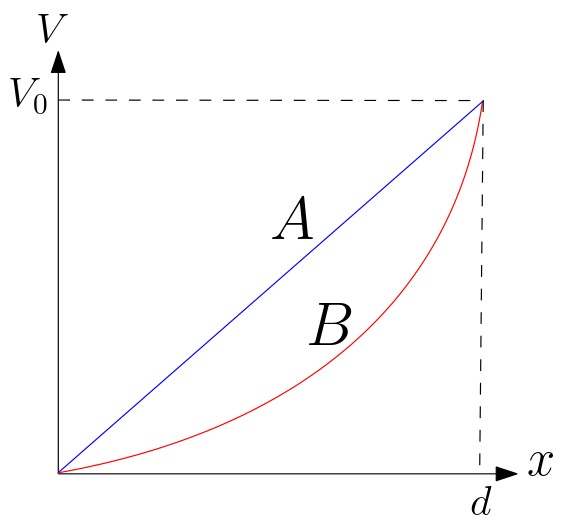
\includegraphics[width = 0.5\linewidth]{PHYS350_Ass3_Fig.png}
		 			\captionsetup{margin=1cm}
		 			\caption{Approximative behaviour of $(3)$ with ($A$) and without ($B$) space-charge.}
		 		\end{figure}
		 	\subsection*{f) }
		 	 	At $x=d$ , $V(x) = V(d) = V_{0}$ therefore, 
		 	 	\begin{align*}
		 	 		V(x) = \left(\frac{9}{4} k\right)^{2/3} x^{4/3} \implies V_{0} &= \left(\frac{9}{4} k\right)^{2/3} d^{4/3} \\
		 	 		&= \left(-\frac{9}{4} \frac{I}{\ep_{0}A} \sqrt{\frac{m}{2q}}\right)^{2/3} d^{4/3} \\
		 	 		V_{0}^{3} &= \frac{81}{16} \frac{I^{2} m }{\ep_{0}^{2} A^{2} 2q} d^{4} \\
		 	 		\therefore I &= \sqrt{\frac{V_{0}^{3}16\ep_{0}^{2} A^{2} 2q}{81 m d^{4}}} 
		 	 	\end{align*}
		 	 	Letting
		 	 	$$ \frac{16 \ep_{0}^{2}A^{2} 2q  }{81 m d^{4}} \equiv K \qquad \implies I = KV_{0}^{3/2}.$$
		 	\section*{Bonus }
		 		\subsection*{a) }
		 			Using Gauss's law for a spherical conductor, 
		 			$$ E = \frac{Q}{4 \pi \ep_{0}r^{2}}, \qquad \text{and} \ \ C = 4\pi \ep_{0}r.$$
		 			Since $Q = CV, $ at a radius $R$ (since $\vec{E} = \vec{0}$ inside the conductor), 
		 			$$ E = \frac{CV}{4 \pi \ep_{0} r^{2}} = \frac{V}{r} = \frac{V}{R}.$$
		 			We have that $R = 0.075 \ \si{\meter}$ and $E_{\text{max}} = 3\times 10^{6} \ \si{\volt\per\meter}$ thus,
		 			\begin{align*}
		 				3 \cross 10^{6} = \frac{V}{0.075} \implies V = 225 000 \ \si{\volt}.
		 			\end{align*}
		 			Moreover, the charge is found with 
		 			$$ Q = CV \implies Q = (4\pi \ep_{0})(0.075)(225 000) = 1.87 \cross 10^{-6} \ \si{\coulomb}.$$
		 		\subsection*{b) }
		 			Let us consider a disk of radius $R$ and a point $P$ on the $x$ axis. Let the charge density be uniform across the disk ,then it follows that $dq = \sigma dA = \sigma 2\pi r \ dr$, such that
		 			\begin{align*}
		 				 dV = \frac{1}{4 \pi \ep_{0}} \frac{dq}{\sqrt{r^{2} + x^{2}}} = \frac{2\pi \sigma r }{4 \pi \ep_{0} \sqrt{r^{2} + x^{2}}} \ dr
		 			\end{align*}
		 			We integrate this expression with respect to the symmetry axis, 
		 			\begin{align*}
		 				V = \int_{0}^{R} \frac{2\pi \sigma r }{4 \pi \ep_{0} \sqrt{r^{2} + x^{2}}} \ dr &= \frac{\sigma}{4 \ep_{0}} \int_{0}^{R} \frac{2r}{\sqrt{r^{2} + x^{2}}}  \ dr \\
		 				&\overset{u = r^{2} + x^{2}}{=} \frac{\sigma}{4 \ep_{0}} \int_{0}^{R} \frac{2}{2} \frac{1}{\sqrt{u}} \ du\\
		 				&= \frac{\sigma}{2 \ep_{0}} \Bigg[\sqrt{r^{2} + x^{2}}\Bigg|_{0}^{R}\Bigg] = \frac{\sigma}{2 \ep_{0}} (\sqrt{R^{2} + x^{2}} - x).
		 			\end{align*}
		 			Since $Q = \sigma \pi R^{2}$ , we conclude that
		 			\begin{align*}
		 				V = \frac{Q}{2 \pi \ep_{0} \pi R^{2}} (\sqrt{R^{2} + x^{2}} - x).
		 			\end{align*}
		 		\subsection*{d) }
		 			Regardless of the mass of the plate it will either stay still given its symmetrical configuration along the sphere, or fly off if it is placed slightly unsymmetrically.
	\end{document}